%%%%%%%%%%%%%%%%%%%%%%%%%%%%%%%%%%%%%%
%%%%%%%%%%%%%%%%%%%%%%%%%%%%%%%%%%%%%%
% Do not edit the TeX file your work
% will be overwritten.  Edit the RnW
% file instead.
%%%%%%%%%%%%%%%%%%%%%%%%%%%%%%%%%%%%%%
%%%%%%%%%%%%%%%%%%%%%%%%%%%%%%%%%%%%%%



We perform a clustering analysis of Fisher's iris data set \textcolor{red}{TODO: cite}. Here each 
data point (with $N=50$ total points)
represents $d=4$ measurements of a particular flower, from one of three
iris species.
We use a standard Gaussian mixture model with conjugate
Gaussian-Wishart prior for the component parameters (detailed in \appref{gmm_example})
and a mean-field VB approximation
 with truncation parameter $\kmax = 15$.
We consider two quantities of interest: (1) $\gclustersabbr$, the posterior expected
number of clusters among the $N$ observed
data points, and (2) $\gclusterspred$, the posterior predictive expected number of clusters in $N$ new (i.e.\ as-yet-unseen) data points.
We set the base stick-breaking prior $\pbase(\nuk)$ to be the standard $\betadist{\nuk \vert 1,\alpha}$
distribution with $\alpha = \alpha_0 = 2$.
Under the base stick-breaking prior with $\alpha_0$, the posterior expected number of clusters
matches the three iris species; see also \figref{iris_fit} in \appref{app_results_iris} for an illustration.

%%
\noindent \textbf{Sensitivity to the concentration parameter}
We approximate the changes in the quantities of interest as $\alpha$ varies
over $\alpha\in[0.1, 4.0]$, which corresponds to an a priori expected number of clusters
among $N$ data points in $[1.5,15]$ (\appref{dp_cluster_growth}). 
Over this range, the shape of a $\betadist{1,\alpha}$
density varies considerably, as shown in
\figref{beta_priors} in \appref{app_results_iris}. 


\begin{knitrout}
\definecolor{shadecolor}{rgb}{0.969, 0.969, 0.969}\color{fgcolor}\begin{figure}[!h]

{\centering 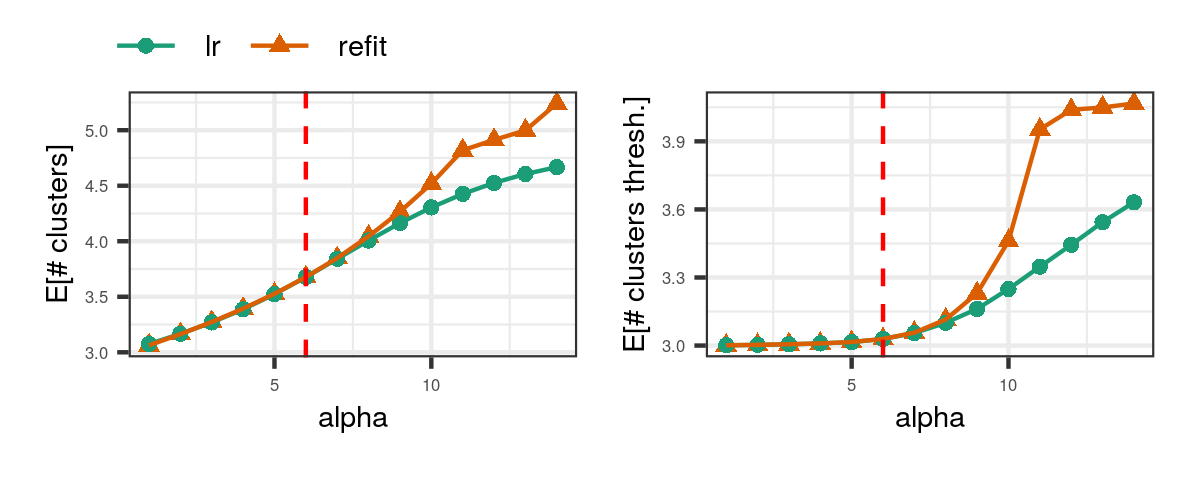
\includegraphics[width=0.784\linewidth,height=0.439\linewidth]{figure/iris_alpha_sens-1} 

}

\caption[The expected number of clusters in the original data set ($\gclustersabbr$, left) and in a new data set of size $N$ ($\gclusterspredabbr$, right) as $\alpha$ varies in the GMM fit of the iris data]{The expected number of clusters in the original data set ($\gclustersabbr$, left) and in a new data set of size $N$ ($\gclusterspredabbr$, right) as $\alpha$ varies in the GMM fit of the iris data. We formed the linear approximation at $\alpha_0=2$.}\label{fig:iris_alpha_sens}
\end{figure}


\end{knitrout}

\Figref{iris_alpha_sens} compares our linear approximation to ground truth
on the two quantities of interest as $\alpha$ varies.
 Over this range of $\alpha$, the posterior expected number of clusters in the observed data 
 is quite robust; it remains nearly constant at three.
 The posterior predictive expected
number of clusters in $N$ new data points is less robust; it ranges roughly from 3.0 to 5.6 expected
species.  Our approximation captures this qualitative behavior. As expected,
the approximation is least accurate furthest from the $\alpha_0$, where the Taylor series
is centered.

%%
\noindent \textbf{Sensitivity to functional perturbations.}
Insensitivity of the expected number of clusters $\gclustersabbr$ to $\alpha$ does
not rule out sensitivity to other prior perturbations. 
We now check how our approximation fares for the multiplicative perturbations in \eqref{mult_perturbation}.
We consider perturbations $\phi$ that are Gaussian bumps in logit stick space, with each
perturbation centered at a different location on the real line.  Each row of
\figref{iris_fsens} corresponds to a different $\phi$. Each $\phi$ is shown in gray
in the leftmost plot of its row. The middle column of
\figref{iris_fsens} shows the stick-breaking prior $\p(\nuk \vert \phi)$ induced
by the corresponding $\phi$.


\begin{knitrout}
\definecolor{shadecolor}{rgb}{0.969, 0.969, 0.969}\color{fgcolor}\begin{figure}[!h]

{\centering 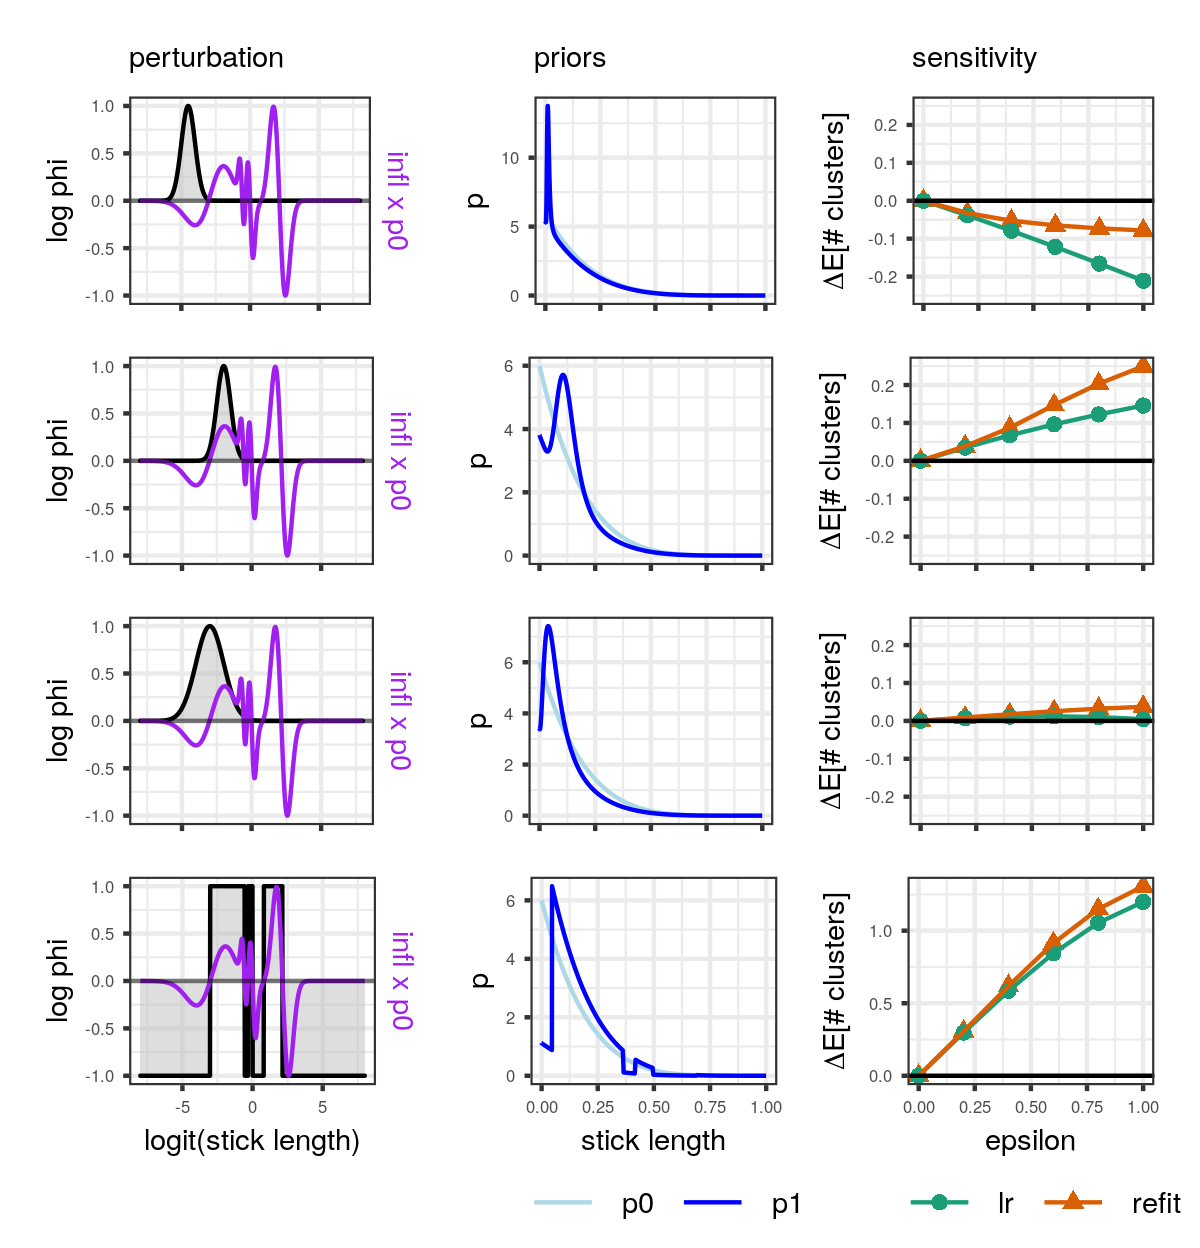
\includegraphics[width=0.980\linewidth,height=0.862\linewidth]{figure/iris_fsens-1} 

}

\caption{Sensitivity of
        the expected number of in-sample clusters
        in the iris data set
        to three multiplicative perturbations each with $\norminf{\phi} = 1$.
        (Left) The multiplicative perturbation $\phi$ is in grey.
        The influence function $\Psi$, scaled so $\norminf{\Psi}=1$, is in purple.
        (Middle) The initial $\pbase(\nuk)$ (light blue)
        and alternative $\palt(\nuk)$ (dark blue) priors. 
        (Right) The effect of the perturbation
        on the change in expected number of in-sample clusters
        for $t \in[0, 1]$.}\label{fig:iris_fsens}
\end{figure}


\end{knitrout}

The rightmost column of \figref{iris_fsens}
shows the changes produced by the $\phi$ perturbation for that row.
We see that our approximation captures the qualitative behavior of the exact
changes.

We also see in this example that we can use the influence function to 
predict the effect of functional changes to the stick-breaking prior.
In the leftmost column, we plot the influence function in the logit space in purple.
According to \corref{etafun_deriv_form}, the sign and magnitude of the effect of
a perturbation should be determined by its integral against the influence
function.  Thus, when $\phi$ lines up with a negative part of $\infl$, as in the
first row, we expect the change to be negative.  Similarly, we expect the
perturbation of the bottom row to produce a positive change, and the middle row,
in which $\phi$ overlaps with both negative and positive parts of the influence
function, to produce a relatively small change. We see this intuition borne out in the
rightmost column.


\begin{knitrout}
\definecolor{shadecolor}{rgb}{0.969, 0.969, 0.969}\color{fgcolor}\begin{figure}[!h]

{\centering 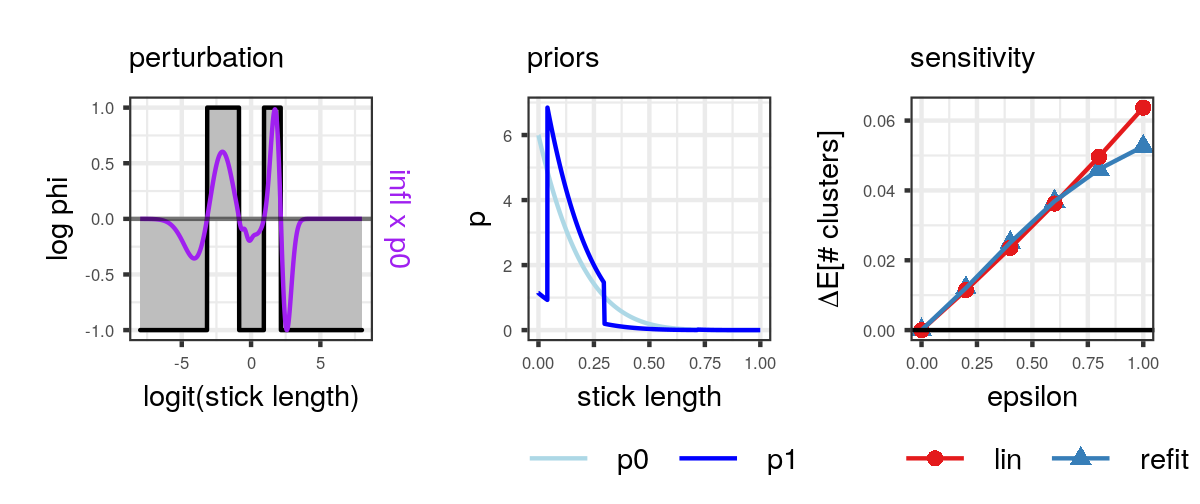
\includegraphics[width=0.980\linewidth,height=0.412\linewidth]{figure/iris_worstcase-1} 

}

\caption[Sensitivity of
        the expected number of in-sample clusters in the iris data set
        to the worst-case multiplicative perturbation with
        $\norminf{\phi} = 1$]{Sensitivity of
        the expected number of in-sample clusters in the iris data set
        to the worst-case multiplicative perturbation with
        $\norminf{\phi} = 1$.}\label{fig:iris_worstcase}
\end{figure}


\end{knitrout}

%%
\noindent \textbf{Worst-case functional perturbation.}
Finally, \figref{iris_worstcase} shows the worst-case multiplicative perturbation with $\norminf{\phi} = 1$, as given by \corref{etafun_worst_case},
along with its effect on the prior and $\gclustersabbr$.
As expected, this worst-case perturbation
has a much larger effect on $\gclustersabbr$
compared to the other unit-norm perturbations in \figref{iris_fsens}.
However, even with the worst-case perturbation---which results in an unreasonably shaped prior density---the change in $\gclustersabbr$
is still small. We conclude that $\gclustersabbr$ appears
to be a robust quantity for this model and dataset.
